\chapter{DreamerV3}

This chapter presents a simplified and mathematically detailed implementation of the DreamerV3 algorithm, drawing inspiration from the paper "DreamerV3: Mastering Diverse Robotic Control by Dreaming"~\cite{ebert2023dreamerv3}.  We aim to provide a clear and understandable representation of the algorithm's core components and their interactions.

\section{World Model: The Agent's Internal Simulator}

The world model \ref{fig:dream}, denoted by parameters $\phi$, learns to predict the future based on current observations and actions. It's the agent's internal simulator, allowing it to "imagine" the consequences of its choices.  We use a Recurrent State-Space Model (RSSM) for this purpose.

\begin{figure}
    \centering
    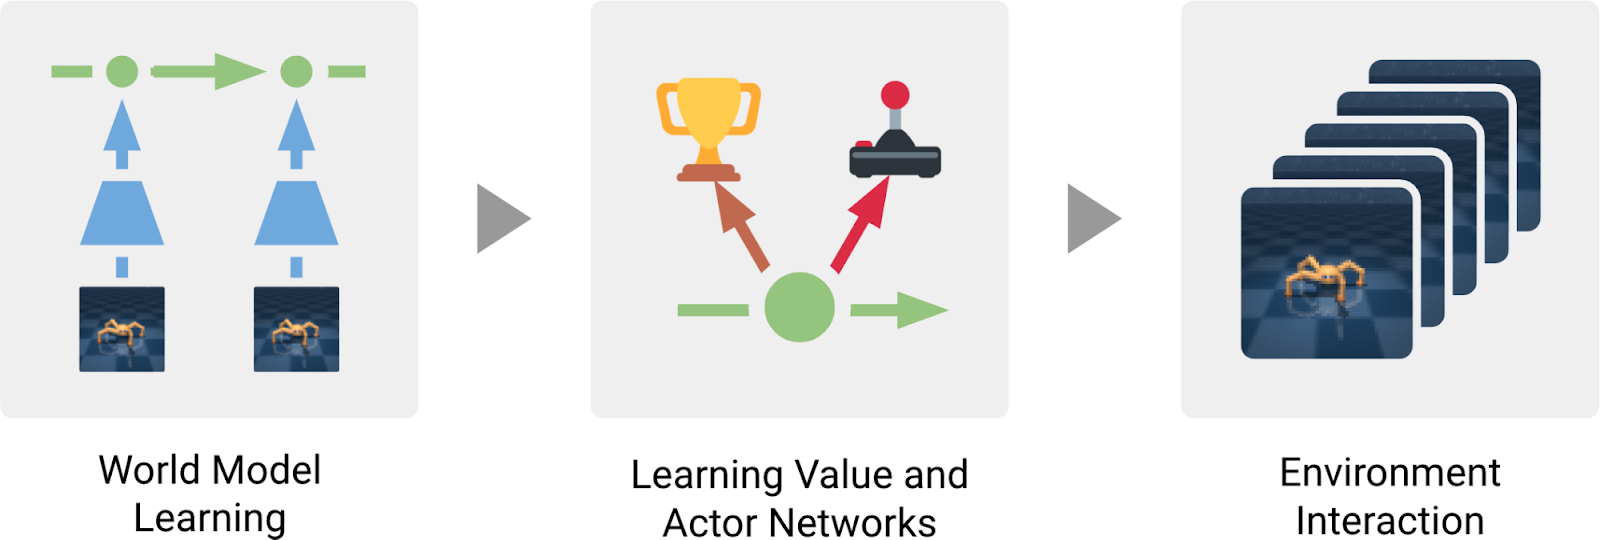
\includegraphics[scale=0.2]{dream}
    \caption{Basic functions of DreamerV3}
    \label{fig:dream}
\end{figure}

\subsection{RSSM Components}

\begin{enumerate}
    \item \textbf{Encoder:} Takes the current observation (sensory input) $x_t$ and the previous hidden state $h_{t-1}$ and produces a latent state $z_t$. This is a probabilistic mapping:
        \begin{equation}
            z_t \sim q_\phi(z_t | h_{t-1}, x_t)
        \end{equation}
        We can think of $q_\phi$ as a neural network (e.g., a multilayer perceptron or a convolutional network if $x_t$ is an image) parameterized by $\phi$.

    \item \textbf{Recurrent Dynamics Model:} Predicts the next hidden state $h_t$ based on the previous hidden state $h_{t-1}$, the previous latent state $z_{t-1}$, and the action taken $a_{t-1}$:
        \begin{equation}
            h_t = f_\phi(h_{t-1}, z_{t-1}, a_{t-1})
        \end{equation}
        $f_\phi$ is another neural network (e.g., an RNN or LSTM).

    \item \textbf{Dynamics Predictor:} Predicts the next latent state $\hat{z}_t$ based on the current hidden state $h_t$:
        \begin{equation}
            \hat{z}_t \sim p_\phi(\hat{z}_t | h_t)
        \end{equation}

    \item \textbf{Reward Predictor:} Predicts the reward $\hat{r}_t$ the agent expects to receive:
        \begin{equation}
            \hat{r}_t \sim p_\phi(\hat{r}_t | h_t, z_t)
        \end{equation}

    \item \textbf{Continue Predictor:} Predicts whether the episode will continue ($\hat{c}_t = 1$) or terminate ($\hat{c}_t = 0$):
        \begin{equation}
            \hat{c}_t \sim p_\phi(\hat{c}_t | h_t, z_t)
        \end{equation}

    \item \textbf{Decoder:} Reconstructs the observation $\hat{x}_t$ from the latent state $z_t$ and hidden state $h_t$:
        \begin{equation}
            \hat{x}_t \sim p_\phi(\hat{x}_t | h_t, z_t)
        \end{equation}
\end{enumerate}

\subsection{World Model Loss}

The world model is trained by minimizing the following loss function:

\begin{equation}
L_{WM}(\phi) = \sum_{t=1}^T \left[ L_{pred}(t) + L_{dyn}(t) + \lambda_{rep} L_{rep}(t) \right]
\end{equation}

where $\lambda_{rep}$ is a weighting factor (e.g., 0.1). The individual loss terms are:

\begin{align}
L_{pred}(t) &= -\log p_\phi(x_t | z_t, h_t) - \log p_\phi(r_t | z_t, h_t) - \log p_\phi(c_t | z_t, h_t) \\
L_{dyn}(t) &= \max\left(1, KL\left(q_\phi(z_t | h_{t-1}, x_t) || p_\phi(z_t | h_t)\right)\right) \\
L_{rep}(t) &= \max\left(1, KL\left(q_\phi(z_t | h_{t-1}, x_t) || p_\phi(z_t | h_t)\right)\right)
\end{align}

The KL divergence term encourages the approximate posterior $q_\phi$ to be close to the prior $p_\phi$. The $\max(1, \cdot)$ term implements the "free bits" technique.

\section{Critic: Evaluating the Agent's Performance}

The critic, parameterized by $\psi$, learns to estimate the expected cumulative reward (return) from a given state. The critic network $v_\psi(s_t)$ takes the state $s_t = (h_t, z_t)$ as input and outputs a prediction of the return.  It is trained to predict the distribution of returns.

The critic is trained using the following loss function:

\begin{equation}
L_C(\psi) = \sum_{t=1}^T -\log p_\psi(R_t^\lambda | s_t)
\end{equation}

where $R_t^\lambda$ is the $\lambda$-return, calculated as:

\begin{align}
R_t^\lambda &= r_t + \gamma c_t \left( (1-\lambda) v_\psi(s_t) + \lambda R_{t+1}^\lambda \right) \\
R_T^\lambda &= v_\psi(s_T)
\end{align}

$\gamma$ is the discount factor, and $\lambda$ controls the balance between bootstrapping and using the actual returns.

\section{Actor: Choosing the Optimal Actions}

The actor, parameterized by $\theta$, learns to select actions that maximize the expected return. The actor network $\pi_\theta(a_t | s_t)$ takes the state $s_t$ as input and outputs a probability distribution over actions. The actor is trained using the following loss function:

\begin{equation}
L_A(\theta) = \sum_{t=1}^T - \frac{R_t^\lambda - v_\psi(s_t)}{\max(1, S)} \log \pi_\theta(a_t | s_t) + \eta H(\pi_\theta(a_t | s_t))
\end{equation}

where $S$ is a running average of the range of returns (between the 5th and 95th percentiles), and $\eta$ is the entropy bonus coefficient.  This loss function combines maximizing returns with encouraging exploration.

\section{Symlog Transformation and Twohot Encoding}

DreamerV3 uses the symlog transformation to handle rewards and observations with different scales. The symlog function is defined as:

\begin{equation}
\text{symlog}(x) = \text{sign}(x) \log(|x| + 1)
\end{equation}

Its inverse, the symexp function, is:

\begin{equation}
\text{symexp}(x) = \text{sign}(x) (\exp(|x|) - 1)
\end{equation}

For rewards and returns, DreamerV3 uses a categorical distribution with exponentially spaced bins and twohot encoding.  This allows the model to predict continuous values while maintaining stable gradients.

This simplified mathematical description provides a more accessible understanding of the DreamerV3 algorithm.  It clarifies the roles of each component and their interactions, highlighting the key mathematical operations involved.  This foundation should be helpful for implementing and adapting DreamerV3 for various robotic control tasks.